\documentclass[11pt]{article}
\usepackage{hyperref}
\usepackage{amsmath, amsfonts, amssymb, mathrsfs, dsfont}
\usepackage{dcolumn}
\usepackage{caption}
\usepackage{subcaption}
\usepackage{filemod}
\usepackage{natbib}
\usepackage[ruled, vlined]{algorithm2e}
\usepackage{floatrow}
\usepackage{setspace}
\usepackage{verbatim}
\usepackage{graphicx}

\hypersetup{
    colorlinks=true,
    linkcolor=blue, 
    urlcolor=black,
    citecolor=blue, 
    }

\oddsidemargin=0.25in
\evensidemargin=0.25in
\textwidth=7in
\textheight=8.75in
\topmargin=-.5in
\addtolength{\oddsidemargin}{-.5in}
\addtolength{\evensidemargin}{-.5in}
\footskip=0.5in
%\doublespacing

\title{Bayesian Deep Gaussian Processes for Correlated Functional Data: \\
        A Case Study in Cosmological Power Spectra}
\author{Stephen A. Walsh\thanks{Corresponding author: Division of Natural Sciences, 
        Math and Technology, Elms College, {\tt walshst@elms.edu}} \and 
        Annie S. Booth\thanks{Department of Statistics, North Carolina State University} \and
        David Higdon\thanks{Department of Statistics, Virginia Tech} \and
        Marco A.R. Ferreira\footnotemark[3] \and
        Kelly Moran\thanks{Los Alamos National Laboratory} \and
        Katrin Heitmann\thanks{Argonne National Laboratory}}
\date{\today}


\begin{document}

\maketitle
\bigskip

\begin{abstract} 
Understanding the structure of our universe and the distribution of matter is an 
area of active research.  As cosmological surveys grow in complexity, the development 
of emulators to efficiently and effectively predict matter power spectra is essential.  
We are particularly motivated by the Mira-Titan Universe simulation
suite which, for a specified cosmological parameterization (termed a ``cosmology''), 
provides multiple response curves of various fidelities, including correlated 
functional realizations.  Our objective is two-fold.  First, we estimate 
the underlying true matter power spectra, with appropriate uncertainty 
quantification (UQ), from all of the provided curves.  To this end, we propose a 
novel Bayesian deep Gaussian process (DGP) hierarchical model which synthesize 
all the information and estimates the underlying matter power spectra, while providing 
effective UQ.  Our model extends previous work on Bayesian DGPs from scalar responses 
to functional ones.  Second, we leverage our predicted power spectra from various 
cosmologies in order to accurately predict the entire matter power spectra for an 
unobserved cosmology.  For this task, we leverage basis function representations 
of the functional spectra to train a separate Gaussian process emulator.  
Our method performs well in synthetic exercises and against the benchmark cosmological 
emulator (Cosmic Emu).  We provide reproducible code in a public git repository.
\end{abstract}

\noindent \textbf{Keywords:} surrogate, computer experiment, uncertainty quantification,
principal components analysis, Mira-Titan, Cosmic Emu (???)

%\vfill

\section{Introduction}
%%%%%%%%%%%%%%%%%%%%%%%%%%%%%%%%%%%%%%%%%%%%%%%%%%%%%%%%%%%%%%%%%%%%%%%%%%%%%%%

%To further our understanding of the structure and movement of the universe, 
%researchers utilize numerous cosmological surveys such as the Sloan Digital Sky 
%Survey \citep{york2000sloan} and the upcoming Nancy Grace Roman Space Telescope 
%\citep{Dore2019WFIRST} which are continuously growing in complexity. With these 
%tools, cosmologists aim to continue learning more about cosmic acceleration 
%\citep{caldwell2009physics}. To this end, one important ingredient to aid in this 
%understanding of our universe is the matter power spectrum. 

Computer simulation experiments are invaluable tools in the study of cosmology.
Experiments which simulate the expansion of the universe are growing
in prevalance and complexity \citep[e.g.,][]{lawrence2010coyote,moran2023mira}
\textcolor{red}{(more cites here?)}.  
We are particularly motivated by a simulation
of the matter power spectrum, which describes the distribution of matter as a 
function of spatial scale. 
%It is often represented as a function of wavenumber $k$ (units Mpc$^{-1}$), which is 
%inversely related to spatial scale. 
On large scales, power spectrum behave according to linear perturbation 
theory \citep{pietroni2008flowing, lesgourgues2009non}.  On smaller scales, nonlinear 
dynamics require the use of computationally intensive simulations, yielding
correlated functional data.
%the Coyote Universe \citep{lawrence2010coyote} and the Mira-Titan Universe \citep{moran2023mira} 
%are two simulation suites dedicated to this effort.  
From the highest level, our aim is to leverage such simulation data to 
first estimate and then predict underlying power matter spectra for various 
cosmological parameterizations.


We are particularly motivated by the Mira-Titan simulation suite \citep{moran2023mira}
which defines ``cosmologies'' according to eight cosmological parameters (\textcolor{red}{more on this
in Section TBD}).  For a particular cosmology, the simulation of the power matter spectra 
is rather complex.  Although we presume there exists some true matter spectra as a function
of wavenumber, we are not able to directly observe it.  Rather, the simulation outputs 
a convoluted patchwork of potential spectra, which vary in fidelity and which are trusted
only over particular wavenumber ranges.  Our first objective is to synthesize expert knowledge
and all of this simulation information into an effective estimate of the true underlying
matter spectrum.

\begin{figure}[ht]
    \centering
    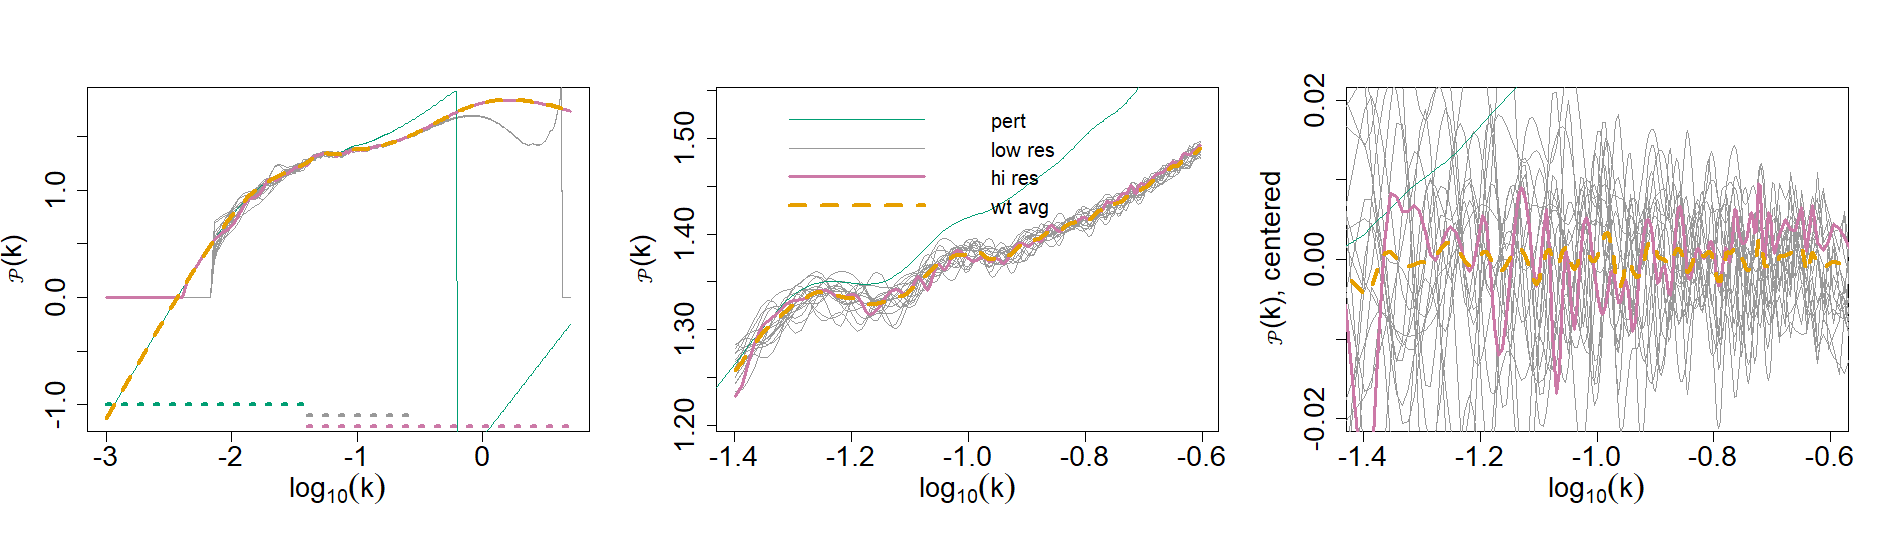
\includegraphics[width=6in]{plot_data.png}
    \caption{Left: The perturbation theory, low resolution runs, and high resolution run 
             for the first training cosmology. The weighted average of these is shown as a dashed line. 
             Dotted lines at the bottom indicate where each data type is deemed approximately unbiased. 
             Right: The same image, but restricted to wavenumber ($k$) values where the low resolution 
             runs are approximately unbiased.}
    \label{fig:plot_data}
\end{figure}

There are several challenges to estimating the underlying spectra.  Our model
must: handle multiple correlated functional observations, offer enough 
flexibility to accommodate the nonstationarity present in power matter spectra 
(which vary in smoothenss across wavenumbers), provide effective uncertainty
quantification (UQ), and allow for the incorporation of expert knowledge 
regarding the wavenumbers over which various outputs are trusted.  To this end, 
we propose a Bayesian hierarchical model which treats each of functional simulation 
output as a realization of a deep Gaussian process \citep[DGP;][]{damianou2013deep} 
centered on the true underlying spectra.  The hierarchical structure naturally
accommodates the correlated observations.  The depth of the GP offers nonstationary
flexibility.  The Bayesian framework facilitates UQ and the incorporation of prior
knowledge.  While Bayesian DGPs have been previously deployed for computer experiments 
with scalar responses \citep[e.g.,][]{sauer2023active,sauer2023vecchia,ming2023deep}, 
they have yet to be extended to correlated functional outputs. 
We will demonstrate profiency on synthetic examples and a low fidelity
cosmological simulation, before deploying our model on the motivating 
Mira-Titan simulation.

Our second objective is to leverage simulation data from a limited set of
cosmologies in order to predict power matter spectra for unobserved cosmologies.
Due to the computationally expensive nature of the Mira-Titan simulation suite
\textcolor{red}{(do we know how long it takes to run?)},
it is infeasible to evaluate the simulation for every possible eight-dimensional
cosmological configuration which may be of interest.  Instead, we desire
a statistical ``emulator'' or ``surrogate model'' 
\citep{santner2003design,gramacy2020surrogates} which will provide quick and effective
predictions of power matter spectra for any cosmological parameterization.
\citet{moran2023mira} provide a state-of-the-art emulator for the Mira-Titan
simulation suite, which was trained on 117 simulations, and is termed 
the ``Cosmic Emu''.\footnote{\url{https://github.com/lanl/CosmicEmu}}
We leverage the same training data, in conjunction with our Bayesian hierarchical
DGP model and basis function representations, to train a Gaussian process surrogate 
on the principal component weights in order to predict spectra for unobserved
cosmologies \citep{higdon2008computer, higdon2010estcosmo}. 
Our method compares favorably to Cosmic Emu on held-out cosmologies.

For a comprehensive assessment of our Bayesian hierarchical DGP model, we 
further study its performance in a simulation study with synthetic data mimicing 
the Mira-Titan data. Additionally, we also train our model with data output from 
the Code for Anisotropies in the Microwave Background \citep[CAMB,][]{lewis2011CAMB};
this model output exhibits similar behavior to Mira-Titan as well, but has the benefit 
of including a ``true" power spectrum corresponding toeach cosmology. 

The remainder of the paper is organized as follows.  Section \ref{sec:data} 
introduces our motivating application, the Mira-Titan simulation suite.  
Section \ref{sec:hm_fit} describes our hierarchical Bayesian DGP model and 
validates its performance on synthetic exercises and the CAMB simulations.  
Leveraging this trained model, Section \ref{sec:pred} details 
our procedure for predicting at unobserved cosmologies, benchmarking against
state-of-the-art competitors on the CAMB and Mira-Titan simulations. 
Section \ref{sec:disc} concludes with a discussion of our contributions and avenues for 
future research.  We provide reproducible code and an R package for our Bayesian DGP model
in a public git repository.\footnote{\url{https://github.com/stevewalsh124/dgp.hm}}
\textcolor{red}{Please note: this repository is currently private until we 
hear back regarding permissions for sharing the Mira-Titan data alongside our code.}

%Leveraging these simulations allows for emulation and prediction of the matter power 
%spectrum under varying specifications for eight different cosmological parameters 
%(i.e., different cosmologies). Estimating and understanding the influence of these 
%parameters on cosmic expansion are areas of active research. In addition to 
%presenting the Mira-Titan simulation suite, \cite{moran2023mira} builds off 
%of previous spectrum emulation \citep{lawrence2017mira} to provide the final 
%emulator (Cosmic Emu) based on the full suite of 117 batches of simulations. 

%In this work, we expand on the previous emulation approaches and propose a 
%novel synthesis of methods to quantify uncertainty and predict matter power 
%spectra for different cosmologies using deep Gaussian processes (DGPs). In order 
%to handle multiple realizations of functional output (from the Mira-Titan 
%simulation suite), we use hierarchical modeling and basis functions within our 
%DGP framework to accurately estimate and predict power spectra for different 
%cosmologies. 

\section{Data}
\label{sec:data}

The Mira-Titan simulation suite is a dataset consisting of simulated power spectra for 
117 different cosmologies. Each of these cosmologies is specified by 8 cosmological 
parameter values, which we will denote as $\theta \in \mathbb{R}^8$. Different simulation 
output exists for different values of a ninth value, the redshift; in this work, we fix 
this value at 0. For each cosmology, we have a batch of 18 simulated spectra: an inexpensive 
spectrum estimated from linear perturbation theory ($y_p$), 16 spectra estimated from 
lower-resolutions simulations ($y_{\ell_r}, r \in \{1,\dots,16\}$), and one spectrum from 
a high resolution simulation ($y_h$). 

These spectra are represented as a function of wavenumber $k$, and hence is denoted $P(k)$. 
Following \cite{moran2023mira}, we model on the emulation space 
$\mathcal{P}(k)=\log_{10}\left(\frac{k^{1.5}P(k)}{2\pi^2}\right)$. The output is available 
for $0.001 \leq k \leq 5$ for $n=351$ different values of $k$, but each data type has differing 
values where it is deemed approximately unbiased. For $k<0.04$, only $y_p$ provides a reliable 
estimate of the spectra. $y_{\ell_r}$ are valid for $0.04 \leq k \leq 0.25$, and $y_h$ is valid 
for $0.04 \leq k \leq 5$. Figure \ref{fig:plot_data} shows an example of the output for a 
particular cosmology.

From the multiple low- and high-resolution spectra across all cosmologies, 
\cite{moran2023mira} obtained precision estimates of these spectra across the $n$ 
wavenumber values ($p_1,\dots,p_n$) using a log-log regression model, and a multiplier 
$c$ for the increase in precision from the low- to high- resolution output. Given 
that the perturbation theory spectra is non-stochastic, we treat this as having a 
precision of $10^5$. We leverage these precision estimates within our model at each 
data type's unbiased wavenumber values to define 
$\Lambda_p = \text{diag}\left((10^5)_{k < 0.04}\right)$, 
$\Lambda_{\ell} = \text{diag}\left(16(p_1,\dots,p_n)_{0.04 \leq k < 0.25}\right)$, 
$\Lambda_h = \text{diag}\left(c(p_1,\dots,p_n)_{0.04 \leq k \leq 5}\right)$. 
Here, each precision matrix is diagonal and the diagonal elements consist of the 
precision values or zero, depending on whether the $k$ value is approximately unbiased 
for that data type. With this, we calculate a weighted average for each cosmology: 
$\bar y = \Lambda^{-1}(\Lambda_p y_p + \Lambda_h y_h + \Lambda_{\ell} \bar{y}_\ell)$, 
where $\Lambda = \Lambda_p + \Lambda_\ell + \Lambda_h$ is the precision matrix for 
the weighted average for a particular cosmology.

We will handle the data in two stages.  First, we will focus on 111 training cosmologies 
and obtain the best estimated spectrum for each.  Second, we will use these estimates 
to predict the spectra for six held-out cosmologies.

\section{Bayesian Hierarchical Modeling for Particular Cosmologies}
\label{sec:hm_fit}

Here we describe our first contribution: the use of a Bayesian hierarchical model 
to estimate the underlying spectra (and quantify uncertainty) for a particular cosmology.  
We focus solely on one cosmology, independent of the others.

\subsection{Gaussian Process Model}

Here, we introduce the Bayesian Gaussian Process (GP) model leveraging the aggregated 
data $D_n \equiv \{X_n, \bar Y, \Lambda\}$ for a particular cosmology. We assume 
the matter power spectrum $S$ for a given cosmology follows a GP with mean $\mu$ 
and covariance matrix $\Sigma_S$.

From plots of the multiple low-resolution spectra (e.g., Figure \ref{fig:plot_data}), 
we find they vary smoothly about some mean $S$, suggesting that a dense covariance 
matrix $\Sigma_\varepsilon$ (accounting for spatial dependence) may outperform a 
diagonal covariance $\Lambda_\ell^{-1}$ for $\bar Y$. In previous work, we have 
modeled multiple candidates for $\Sigma_\varepsilon$ \citep{walsh2023bayesian} and 
found that a Mat\'ern covariance $\Sigma_\ell$ trained on the low-resolution runs 
(pre-scaled by the precision values and subtracting a LOESS-smoothed average) performs 
the best. We specify this structure within $\Sigma_\varepsilon$ and refer readers 
to \cite{walsh2023bayesian} for a more detailed exposition. This yields 
$\Sigma_\varepsilon=\left(\Lambda_p^{-1} + \Sigma_\ell + \Lambda_h^{-1}\right)^{-1}$, 
where $\Lambda_p, \Sigma_\ell^{-1}, \text{ and } \Lambda_h$ are all $n\times n$ 
and are 0 wherever the corresponding data type is biased.

We transform $X$ values to fall within $[0,1]$ and $Y$ so that the mean and variance 
are 0 and 1, respectively. This allows for a straightforward specification of priors, 
where the hyperparameters for the Mat\'ern covariance $\Sigma_S$ each take a vague prior. 
Specifically:

\begin{align}
\Sigma_\ell^{i,j} = \tau_\ell^2  \left( 1 + \frac{\sqrt{5}d}{\sqrt{\theta_\ell}} + 
  \frac{5d^2}{3\theta_\ell}\right) \exp\left(-\frac{\sqrt{5}d}{\sqrt{\theta_\ell}}\right),\\
\Sigma_S^{i,j} = \tau_S^2  \left( 1 + \frac{\sqrt{5}d}{\sqrt{\theta_S}} + 
  \frac{5d^2}{3\theta_S}\right) \exp\left(-\frac{\sqrt{5}d}{\sqrt{\theta_S}}\right),
\end{align}

where $d=||x_i-x_j||^2$. From here, we estimate $\tau_\ell, \theta_\ell$ with maximum 
likelihood, and conditional on $\Sigma_\varepsilon$, we specify priors for $\tau_S, \theta_S$ 
following \cite{sauer2023active}: \textcolor{cyan}{Annie, please ensure the most up-to-date 
prior specs are shown above and here. Here is what I found from fit\$settings when using 
deepgp v1.1.3: $\theta_S \sim G(\alpha=1.2, \beta=1)$ and $\tau_S \propto 1/\tau_S^2$.}

% $$
% \mathbf{\Sigma_\varepsilon} =
% \begin{bmatrix}
% \Lambda_p^{-1} & \mathbf{0} & \mathbf{0} \\
% \mathbf{0} & \mathbf{\Sigma}_{\ell} & \mathbf{0} \\
% \mathbf{0} & \mathbf{0} & \Lambda_h^{-1}
% \end{bmatrix}
% $$

Therefore, we model $\bar Y|S$ as a GP with mean $S$ and block-diagonal covariance 
matrix $\Sigma_\varepsilon$:

\begin{align}
\bar Y|S &\sim \mathcal{N}_n(S,\Sigma_\varepsilon) \\
S &\sim GP\left(\mu, \Sigma_S(x,x')\right)
\end{align}

Upon integrating out $S$, we obtain $\bar Y \sim \mathcal{N}_n(\mu, \Sigma_S+\Sigma_\varepsilon)$. 
Additionally, this model yields the posterior distribution $S|\bar Y \sim \mathcal{N}_n(m, C)$, 
where $C=\left(\Sigma_S^{-1}+\Sigma_\varepsilon^{-1}\right)^{-1}$ and 
$m=C\left(\Sigma_\varepsilon^{-1}\bar Y+\Sigma_S^{-1}\mu\right)$. 
This distribution provides the posterior mean and corresponding uncertainty for 
$S$ within a given cosmology. 
% With this hierarchical model, we improve the efficiency of estimating $S|\bar{Y}$.

\subsection{Deep Gaussian Process Model}

Considering the Mira-Titan data, some nonstationarity is expected (e.g., due to 
baryonic acoustic oscillations when $-2 \leq \log_{10}(k) \leq -1$). To account 
for this, we incorporate a latent layer $W$ within the hierarchical model to warp 
locations of $X$ and incorporate nonstationary dynamics of the matter power spectra. 
When $W$ is a GP, this creates a deep Gaussian process (DGP) model \citep{damianou2013deep}. 
Additional latent layers could be considered, although one is sufficient for this 
dataset \citep{dunlop2018deep}.

\begin{align}
\bar Y|S,W &\sim \mathcal{N}_n(S,\Sigma_\varepsilon) \\
S|W &\sim GP\left(\mu, \Sigma_S(w,w')\right) \\
W &\sim GP\left(0, \Sigma_W(x,x')\right)
\end{align}

We have found that whether the prior mean of $W$ is set to 0 or $X$ 
\citep[which would indicate stationarity apriori,][]{schmidt2003bayesian} does not 
have a substantial impact on the model fit. We construct this model in the 
compositional form, and also use Markov Chain Monte Carlo (MCMC) to estimate and 
obtain full uncertainty for each of the model parameters \citep{sauer2023active}.

\textcolor{cyan}{Annie: want to add something here? For $\theta_w$, we also specify 
a Gamma prior of the form $\theta_w \sim G(\alpha=1.2, \beta=2)$. We discuss the 
elliptical slice sampling of $W$, but otherwise it is plugged in to the methods 
of the previous section with very few changes.}

Through the synthesis of the DGP model alongside the additional level of hierarchical 
modeling (HM) to incorporate multiple functional model runs, we call this method DGP.HM.

\subsection{Simulation Study}
\label{subsec:sim}

We compare DGP.HM to competing models with a simulation study where the underlying 
true curve is known. Following \cite{moran2024dpc}, we consider two functions 
($f_1$ and $f_2$) each with two variance specifications (settings ``4" and ``5", 
\textcolor{magenta}{we can consider additional homoskedastic cases in the appendix if necessary}). 

Here, $f_1$ and $f_2$ are defined as follows:
\begin{align}
  f_1(x) &= m_1 \exp(-u_1x/2) * \cos(wx) - m_1x/5, \quad w=\sqrt{25-[u_1/2]^2} \\
  f_2(x) &= \exp(-m_2[x-3]^2)+\exp(-u_2[x-1]^2)-0.05\sin(8[x-1.9]), \\ 
  \quad x &\in [0,4].
\end{align}

For additional variation, the values of $m_1, m_2, u_1,$ and $u_2$ are random where 
$m_1 \sim \text{Uniform}(0.5,1.5)$, $u_1 \sim \text{Uniform}(1.5,2.5)$, and $m_2,u_2 
\sim \text{Uniform}(0.6,1.4)$. 
      
For the two variance settings, we consider matrices $\Sigma_4$ and $\Sigma_5$ to 
have a Mat\'ern covariance function with a nugget of $10^{-8}$ and smoothness of 2.5. 
For setting ``4", we have $\tau^2=0.0225$ and $\theta=0.01$. For setting ``5", we have 
$\tau^2=0.01$ and $\theta=0.05$, and additionally scale this covariance matrix by 
a vector of values $s$ so that $\Sigma_5 = s M s^T$ is nonstationary; here $M$ is 
a Mat\'ern covariance matrix with parameters $\tau^2$ and $\theta$.

For each simulated function and variance specification, we generate 20 values of 
$m_1, m_2, f_1, f_2$, and conditional on these values, we sample either 5 or 20 
functional observations and estimate the underlying true function based on the observations.

\begin{figure}[t]
    \centering
    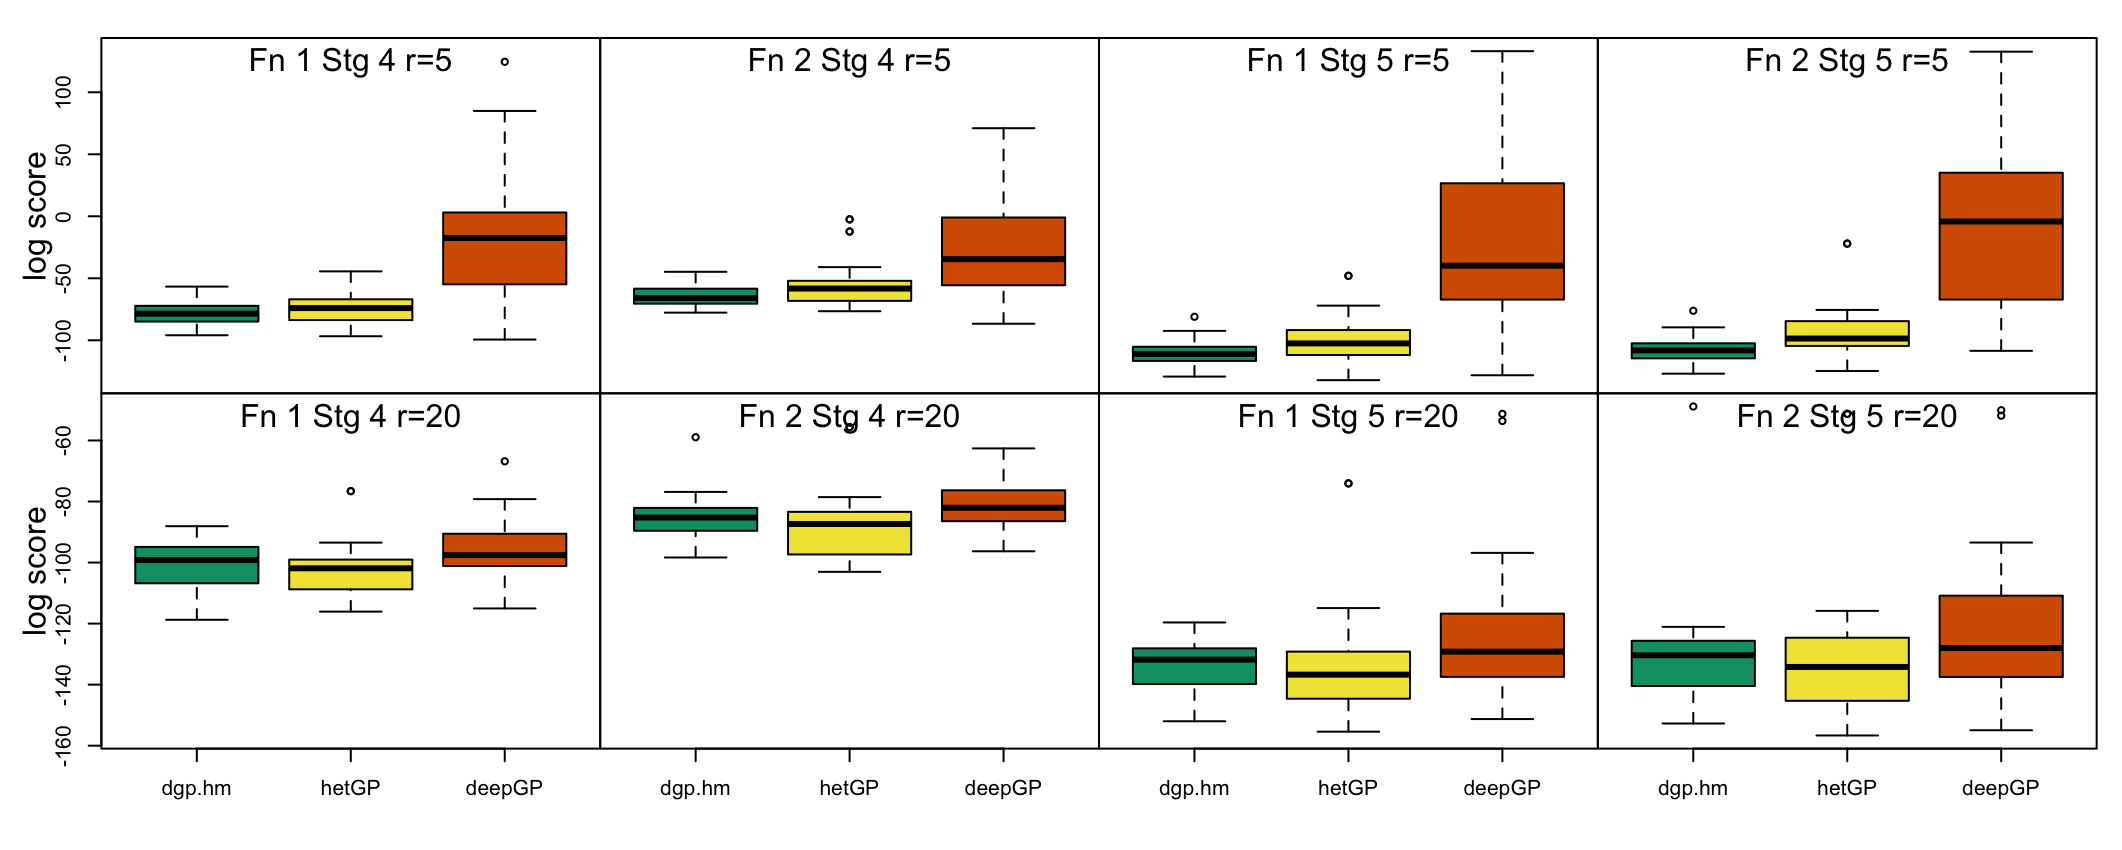
\includegraphics[width=6in]{sims_logS.png}
    \caption{Boxplot of log scores across two different functions and covariance 
             settings (lower is better). For each case, the boxplot is constructed 
             from 20 random batches were simulated. Each column represents a function/variance 
             specification pair, and each row shows results for batch sizes of either 
             5 (top) or 20 (bottom).}
    \label{fig:sims_logS}
\end{figure}

The competing methods we consider are an out-of-the-box DGP fit using the 
\texttt{deepgp} package \citep{sauer2023active}, a heteroskedastic GP fit using 
the \texttt{hetGP} package \citep{binois2018practical, binois2021hetgp}, as well 
as a deep process convolution (DPC) approach, which is utilized within Cosmic 
Emu \citep{moran2023mira}. 

The metrics we use to evaluate performance are mean squared error (MSE) and the 
log score, a proper scoring rule which takes both prediction and intervals into 
consideration \citep{gneiting2007strictly}. For both metrics, a lower value indicates 
better performance. Log score and MSE results are shown in Figures \ref{fig:sims_logS} 
and \ref{fig:sims_MSE} respectively; our DGP.HM model performs favorably against 
these current benchmark methods. \textcolor{magenta}{If we mention that DGP.HM timings 
speed up compared to \texttt{deepgp}, we would also need to mention that \texttt{hetGP} 
is much faster than both of these.}

\begin{figure}
    \centering
    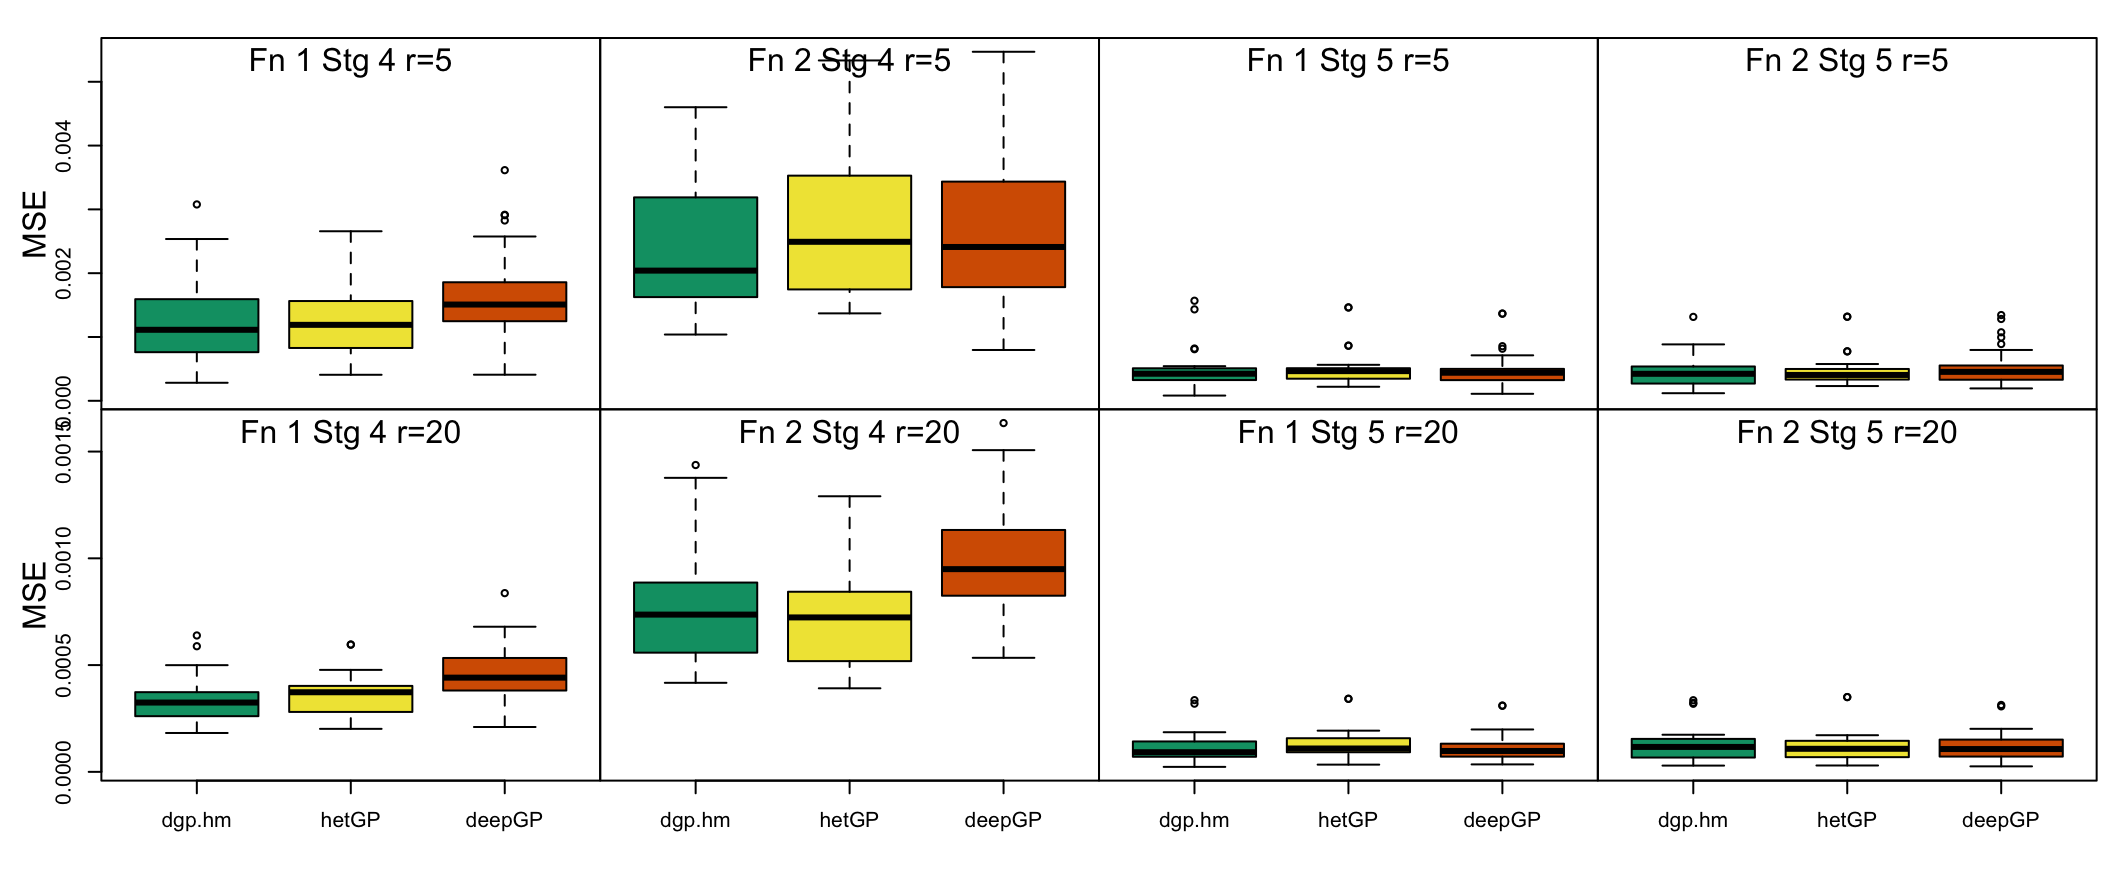
\includegraphics[width=6in]{sims_MSE.png}
    \caption{Boxplot of MSEs across two different functions and covariance settings 
             (lower is better). For each case, the boxplot is constructed from 20 
             random batches were simulated. Each column represents a function/variance 
             specification pair, and each row shows results for batch sizes of 
             either 5 (top) or 20 (bottom).}    
    \label{fig:sims_MSE}
\end{figure}

\subsection{CAMB Data}
\label{subsec:camb}

In addition to simulated data, we investigate model fits for different cosmological 
datasets from CAMB \citep{lewis2011CAMB}. \textcolor{magenta}{We have looked at two sets of model 
runs, ``LT" runs where there is an underlying ``true" value alongside 15 computer 
model runs, or the ``CAMB" runs, where we only have a single output. The performance 
from the CAMB runs was better (with a 6-dimensional design space), and also did not 
require obtaining a posterior mean from multiple model runs. When looking at the 
CAMB runs on the $\Delta$ space, we see it generally is withing $\pm 5\%$ error. 
Regarding these results, compared to the results for the 8-dimensional LT runs 
which had less impressive predictive performance, I'm open to suggestions on whether 
to include details on one or the other.}

\begin{figure}
    \centering
    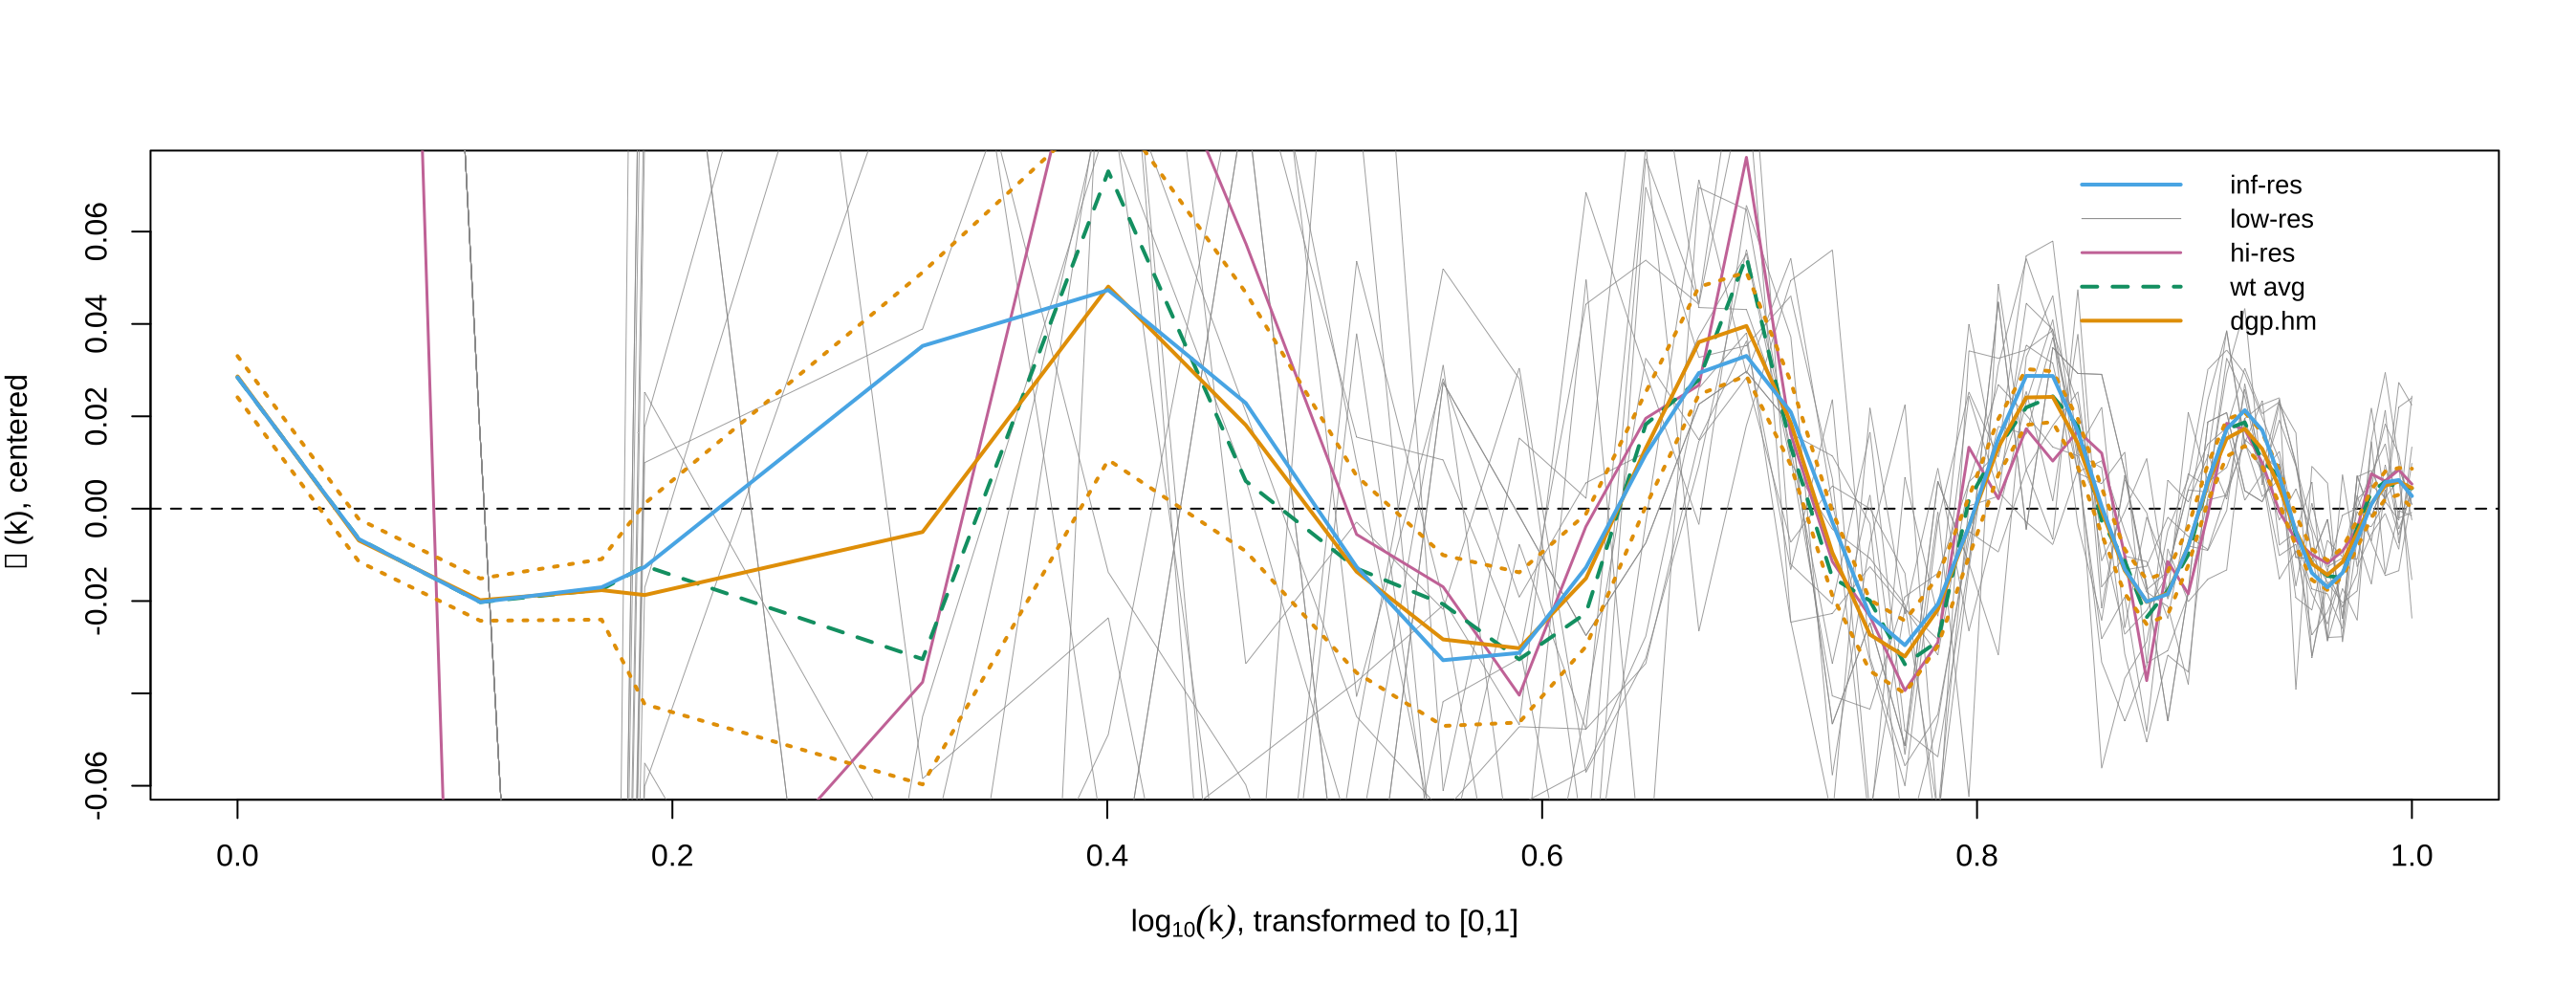
\includegraphics[width=6in]{CAMB_fit_model1.jpg}
    \caption{Example of model fit for the first model from the CAMB data, with LOESS
             mean term subtracted. \textcolor{red}{Steve: Update this plot to be
             more clean, use different line types: dotted, dash, solid, etc.}}   
    \label{fig:fit_camb}
\end{figure}

\begin{figure}
    \centering
    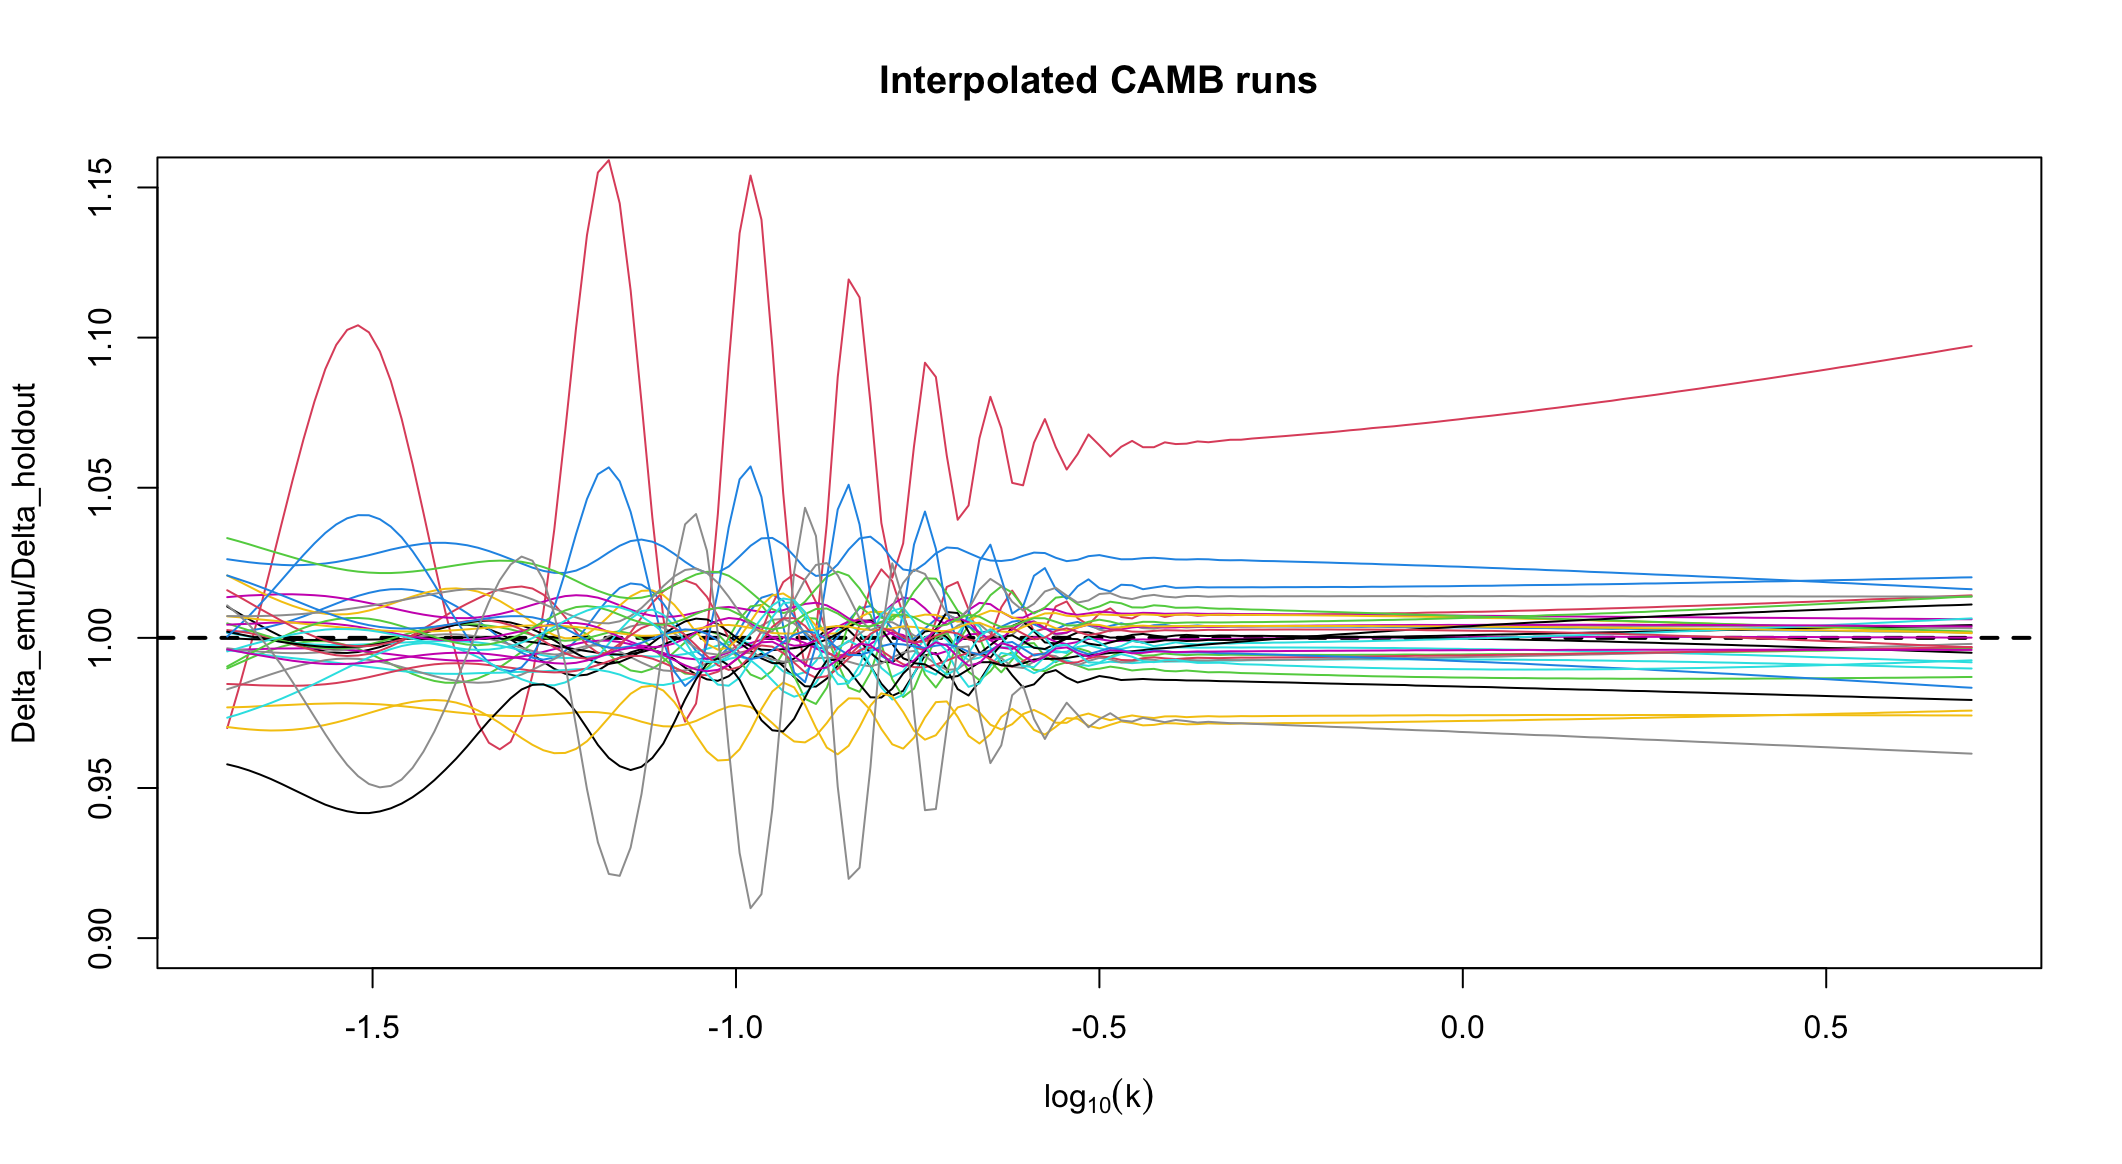
\includegraphics[width=6in]{plot_pca_CAMB.png}
    \caption{Proportion of $\Delta_{emu}$ vs. $\Delta_{holdout}$ for model 
             runs 11-42 (excluding 27-28).}   
    \label{fig:pca_camb}
\end{figure}

\subsection{Estimating Spectra with Mira-Titan Data}
\label{subsec:mira_fit}

To train our hierarchical model, we initialize our hyperparameter estimates across 
all cosmologies by modeling the first (M001) with 50,000 MCMC runs, and use these 
as initial values for all cosmologies. Specifically, we save the last MCMC 
iteration of $W$, $\theta_w$ and $\theta_S$ as $W_0$, $\theta_{w0}$ and $\theta_{S0}$ 
respectively and use each as starting values for all 111 training cosmology fits, 
where each cosmology is fit with 10,000 MCMC runs (5,000 removed as burn-in and 
every 5th sample is kept, resulting in 1,000 posterior samples).

From these samples, we can estimate and quantify the uncertainty within each 
cosmology's average and latent layer $W$. Figure \ref{fig:plot_fit} shows an 
example of the uncertainty for our posterior mean for the first (of 111) training 
cosmologies; the posterior mean is subtracted in order to visualize this uncertainty. 
Figure \ref{fig:plot_warp} provides elliptical slice samples of $W$ along with the 
average warping. Some departure from stationarity is estimated in the higher $X$ 
(i.e., scaled $k$) values.

\begin{figure}[ht]
    \centering
    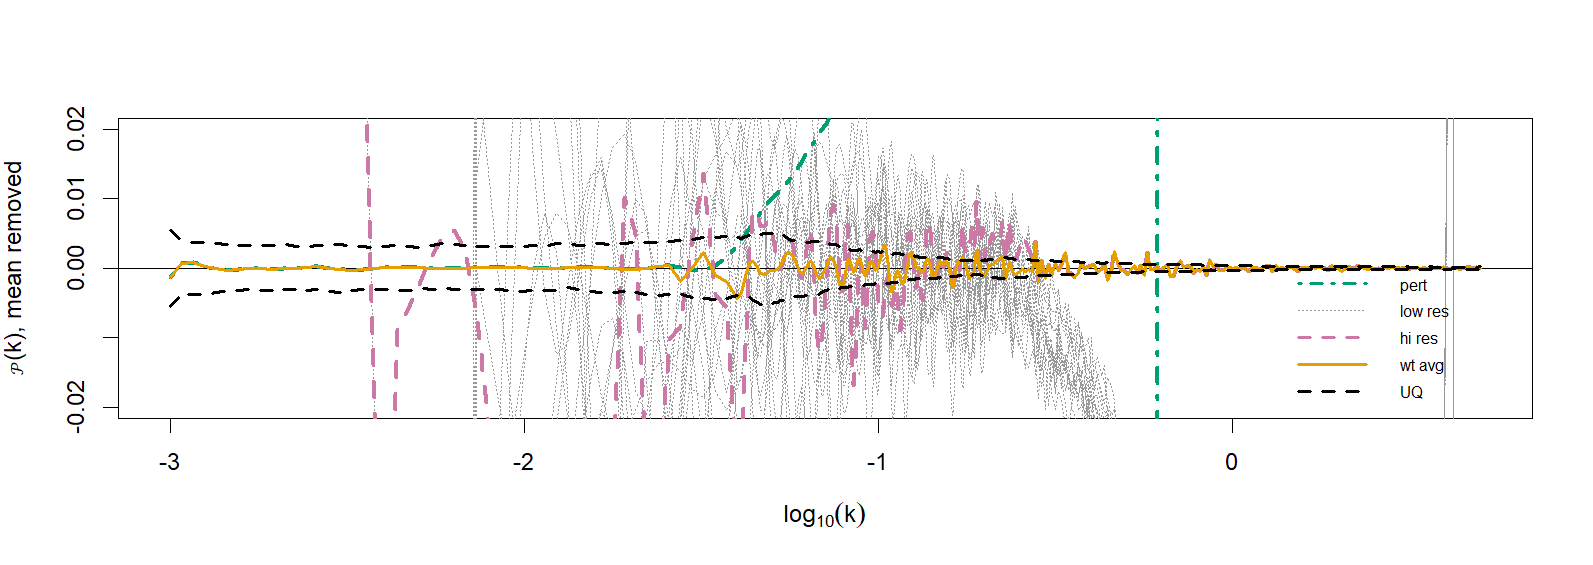
\includegraphics[width=6in]{plot_fit.png}
    \caption{95\% credible intervals for the power spectrum of model 1 (posterior mean 
             subtracted). Plots of the perturbation theory, low-resolution and high-resolution 
             runs are also shown, alongside the weighted average.}
    \label{fig:plot_fit}
\end{figure}

\begin{figure}[ht]
   \centering
   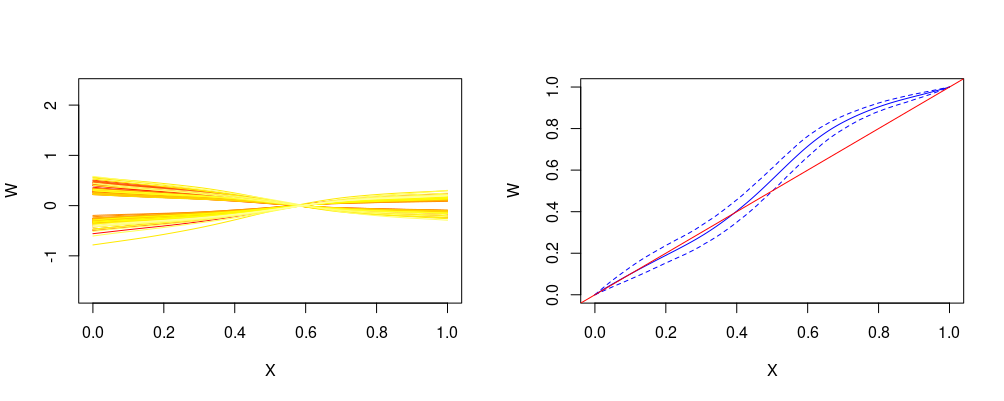
\includegraphics[width=6in]{plot_warp_M001.png}
   \caption{Left: MCMC samples of $W$ for model M001 after burnin and thinning. 
            Right: Corresponding 95\% credible intervals for $W$, where departure 
            from the identity line represents nonstationary behavior.}
   \label{fig:plot_warp}
\end{figure}

\section{Prediction for Unobserved Cosmologies}
\label{sec:pred}

Upon obtaining the posterior means from each of the 111 training cosmologies, this 
section details our second contribution - the use of the Bayesian DGP.HM model 
to predict the curve for held-out cosmologies. This is achieved with modeling the 
weights of different basis functions as GPs.

\subsection{GP-PC Model}
\label{subsec:pca}

Here, we begin with a $n \times m$ matrix composed of $m=111$ posterior means, 
each of length $n$, denoted by $\boldsymbol\eta$. To facilitate more efficient estimation, 
we use singular value decomposition \citep[SVD; e.g.,][]{banerjee2014linear}, 
where $\boldsymbol\eta = UDV^T$; $U$ and $V$ are orthogonal matrices of size $n \times n$ 
and $m\times m$, respectively. $D$ is a diagonal matrix containing the singular values. 
For this application, $\boldsymbol\eta$ has rank $r=\text{min}\{m,n\}=111$, which 
determines the number of non-zero elements in $D$. We find an alternative decomposition 
where $\Sigma$ is a diagonal matrix with the non-zero singular values of $\boldsymbol\eta$, 
and $U_1$ and $V_1$ are matrices with orthonormal columns of size $n_\eta \times r$ 
and $m \times r$, respectively. 

Following \cite{higdon2008computer, higdon2010estcosmo}, we equivalently decompose 
$\boldsymbol\eta$ into a principal component (PC) basis matrix 
$B^* = \frac{1}{\sqrt{m}}U_1\Sigma$ along with its corresponding weights 
$W^* = \sqrt{m}V_1$. Without loss of generality, we can perform this decomposition 
after an overall mean trend is removed. If we use $p_\eta < r$ PCs, this will reduce 
$B$ and $W$ to be the first $p_\eta$ columns of $B^*$ and $W^*$ respectively and 
result in an approximation where 

\begin{equation}
    \boldsymbol\eta= UDV^T = U_1\Sigma V_1^T \approx BW^T.
\end{equation}

Figure \ref{fig:mean_PCs_oneW} illustrates this decomposition with the estimated 
mean trend, the principal components contained in $B$, and one example of how the 
weight for the first PC will vary dependent on the first of $p_\theta=8$ cosmological 
parameters contained in $\theta$.

In the following subsections, we consider different modeling strategies for $W$, 
which will influence predictions and sensitivity analyses based on $\boldsymbol\eta$.

\begin{figure}
    \centering
    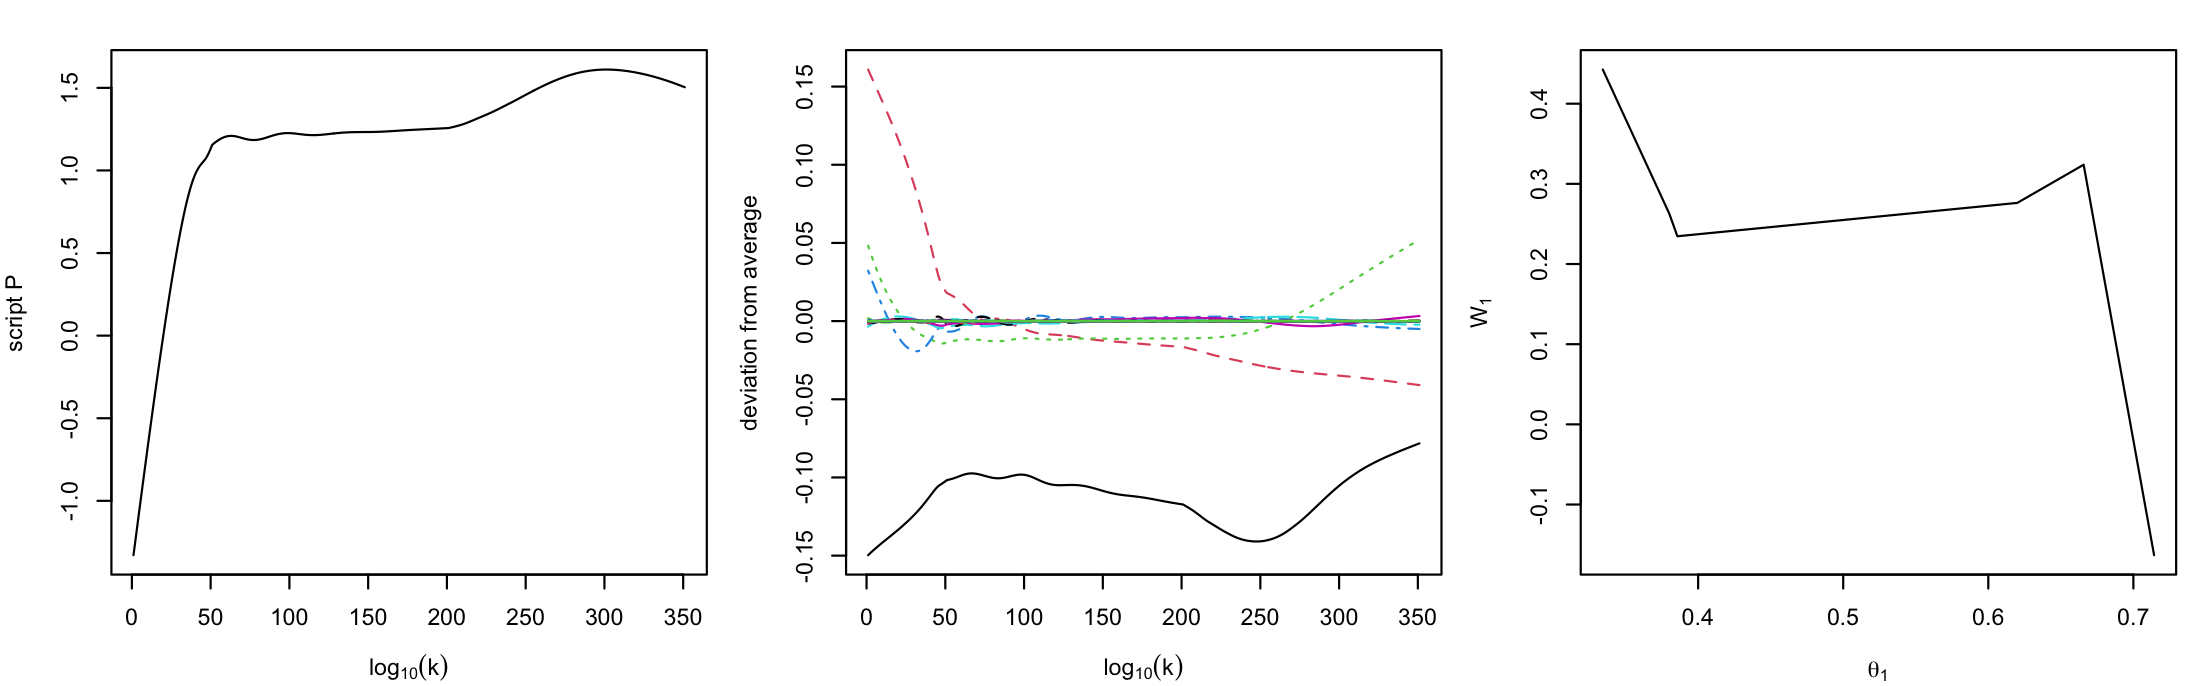
\includegraphics[width=\textwidth]{mean_PCs_oneW.png}
    \caption{The estimated mean trend of the 111 posterior means (left), the principal 
    components contained in $B$ (middle), and an illustration of how the weights 
    for the first PC will change as the first cosmological parameter varies (right) 
    \textcolor{red}{This last plot is wonky because it was made with only the 6 test 
    cosmologies, not a large uniform or FF design, Steve can update this}.}
    \label{fig:mean_PCs_oneW}
\end{figure}


In alignment with \cite{heitmann2009coyote} and \cite{higdon2010estcosmo}, we use 
GPs to model the principal components' weights; we shall denote this method GP-PC. 
We assume a powered exponential kernel for the Gaussian process and employ 
\texttt{GPfit} to perform a multi-start gradient based search for GP's hyperparameters 
\citep{macdonald2015gpfit}. That is, the $i$th vector of PC weights $w_i(\theta)$, 
$i \in \{1,\ldots,p_\eta\}$, will be modeled as a zero mean GP: 
$w_i(\theta) \sim GP(0, \sigma^2R)$, with

\begin{equation*}
    R_{ij} = \prod_{k=1}^{p_\theta}\exp\left\{-10^{\beta_k}|x_{ik}-x_{jk}|^\alpha\right\}
\end{equation*}

We fix $\alpha=1.95$ and estimate each $\beta_k$ with $k \in \{1,...,p_\theta\}$. 
Using these trained GPs from the PCs, we predict the spectra for unobserved cosmologies.

\subsection{Predicting Spectra from Mira-Titan Data}
\label{subsec:mira_pred}

Here we show prediction results for 6 held-out cosmologies. We compare our method 
with Cosmic Emu \citep{moran2023mira}, the emulator constructed using the full suite 
of 111 Mira-Titan model runs. Cosmic Emu uses a Bayesian approach where the smooth 
spectrum for each cosmology is modeled with a process convolution on Brownian motion. 
Nonstationarity is permitted through modeling the bandwidth parameter with a process 
convolution as well; this composition is referred to as a deep process convolution 
\citep{moran2024dpc}.

Both Cosmic Emu and DGP.HM are capable of modeling a true underlying functions based 
upon multiple functional realizations, but our approach utilizes DGPs within a 
hierarchical model in lieu of deep process convolutions. After obtaining the estimated 
smooth spectra from the training cosmologies, each method utilizes GPs in order to 
estimate the weights of the PCs from the estimated spectra. Below, we compare prediction 
performance between Cosmic Emu and DGP.HM for the 6 held-out cosmologies. 
\textcolor{magenta}{In addition, we can also predict over a large uniform or full 
factorial design to obtain estimated main effects for each cosmological parameter in 
$\theta$, interactions amongst the $p_\theta=8$ parameters, and decompose the overall 
variation by main effects, two-way interactions, and so on. Should this be included?}

Plots for the average root mean squared error (RMSE) for each prediction method over the 
6 cosmologies and each $k$ value are shown in Figure \ref{fig:plot_rmse_k}. Comparisons 
of the spectrum estimation for training cosmologies are shown as well (using RMSE against 
the weighted average of observations). For predictions, DGP.HM achieves the greatest 
reduction in RMSE in the region where perturbation theory and the low-resolution runs 
are deemed unbiased. For the region where only the high-resolution run is unbiased, 
Cosmic Emu has a lower average RMSE. Over all $k$ values and predictions, DGP.HM has 
an average RMSE of 0.0089 and Cosmic Emu has an average RMSE of 0.0106. Our RMSE is 
lower at 56\% of $k$ values considered. The individual predictions for each method and 
cosmology are shown in Figure \ref{fig:plot_pred_1to6}.

\begin{figure}[ht]
    \centering
    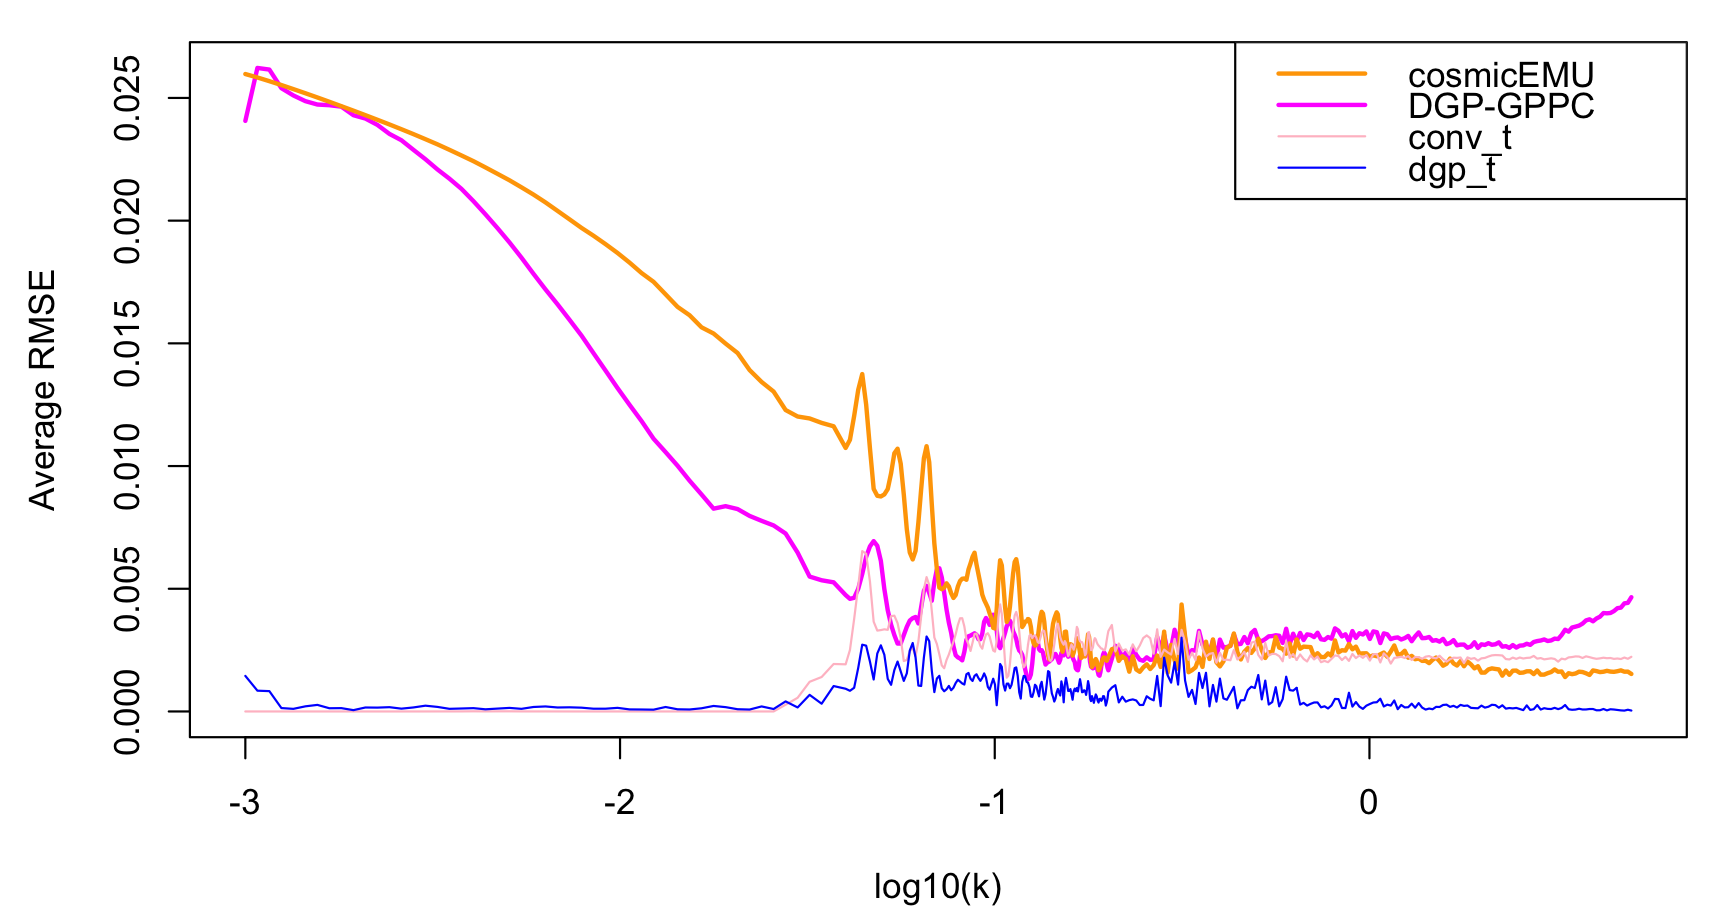
\includegraphics[width=6in]{rmse_by_k.png}
    \caption{Left: Average RMSE of each prediction method across all $k$ values. 
             Right: Average RMSE for each method when using the held-out computer 
             model runs to train the model. In each case, the truth is assumed to 
             be the weighted average of the computer model runs.}
    \label{fig:plot_rmse_k}
\end{figure}

% \begin{figure}[ht]
%     \centering
%     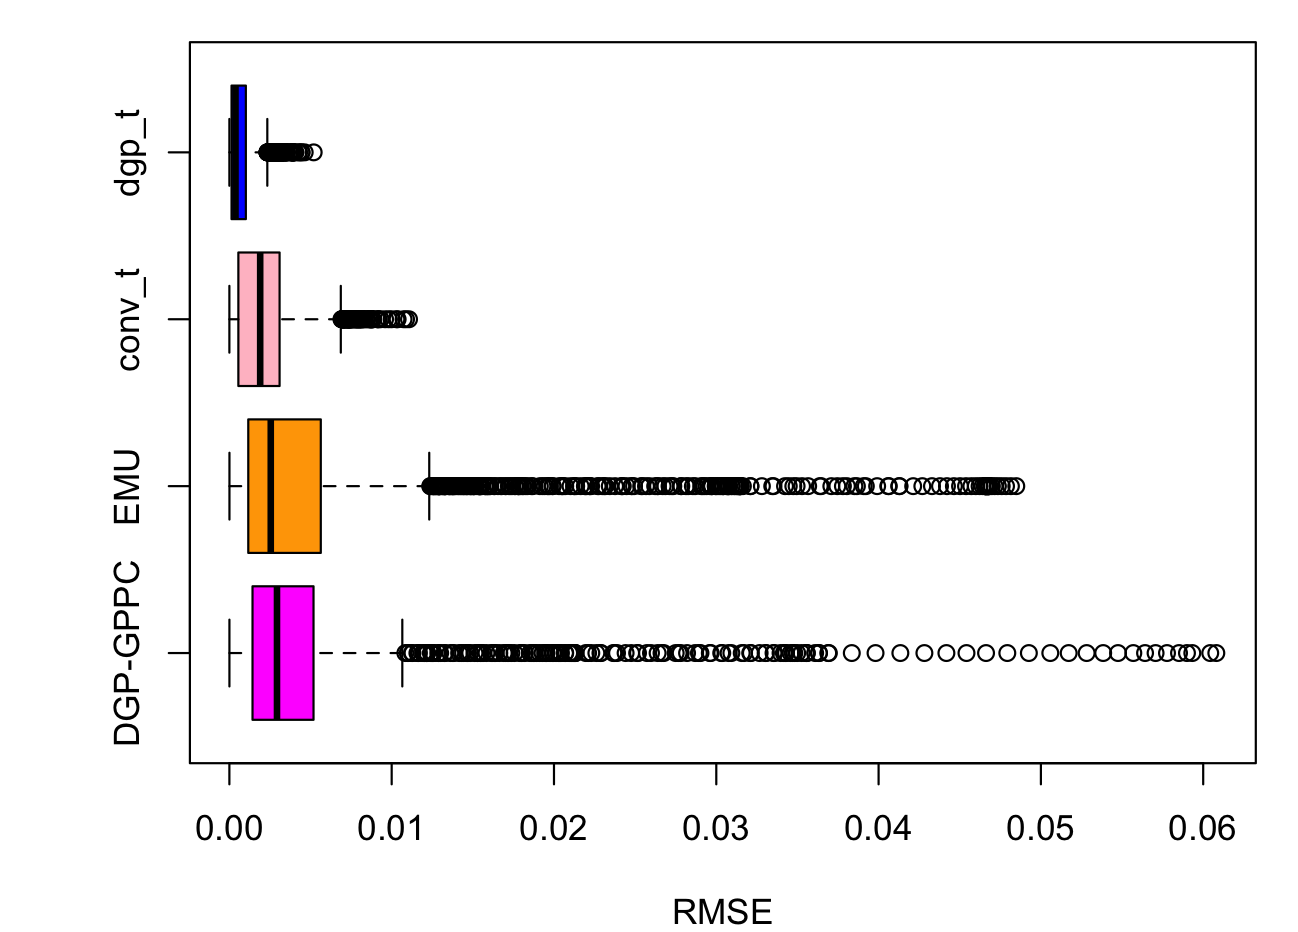
\includegraphics[width=6in]{rmse_box.png}
%     \caption{Boxplot of all RMSEs of each method across all six test models. 
%.             From top to bottom: box plots for our training method, process 
%              convolution training method, Cosmic EMU predictions, and our DGP-PC predictions.}
%     \label{fig:plot_rmse_box}
% \end{figure}

\section{Discussion}
\label{sec:disc}

In this work, we propose a novel Bayesian hierarchical model which utilizes DGPs 
in order to estimate a smooth underlying function from correlated functional observations 
(as cosmological computer model runs). In addition to the compositional form of the DGP, 
we include a third component modeling the correlated errors for each spectrum. 
With all smooth spectra estimated from the training set of 111 batches of model runs, 
we can predict spectra for unobserved cosmologies.

Multiple avenues for future research emerge: in addition to estimating dark matter 
power spectra, batches of hydrodynamical simulations exist, and this method could 
easily be adapted to handle such datasets. Other applications outside of cosmology 
can be explored, wherever multiple functional outputs exist, perhaps with spatial 
correlation (for example, observing multiple tropical cyclone forecasts). More detailed 
sensitivity analyses for the cosmological parameters can be explored to gain insights 
into how each of these parameters interact, and which are most significant. From a 
modeling perspective, changes to the model could include modeling the latent layer 
$W$ jointly across different cosmologies, as well as considering different redshift 
values other than $z=0$. Leveraging a hybrid model between DGP.HM and Cosmic Emu 
may also help to obtain accurate estimates on the lower and higher ends of $k$ values, 
respectively. Additionally, Bayesian smoothing spline ANOVA (BSS-ANOVA) or other methods 
could be compared in addition to DGPs. 

\section{Appendix}
\label{sec:apdx}

\textcolor{magenta}{The different appendices from dissertation as necessary. 
Can also put details of dataset in supplementary material.} 
\textcolor{red}{Fix references as necessary, e.g. Moran et al. 2024.}

\begin{figure}[ht]
    \centering
    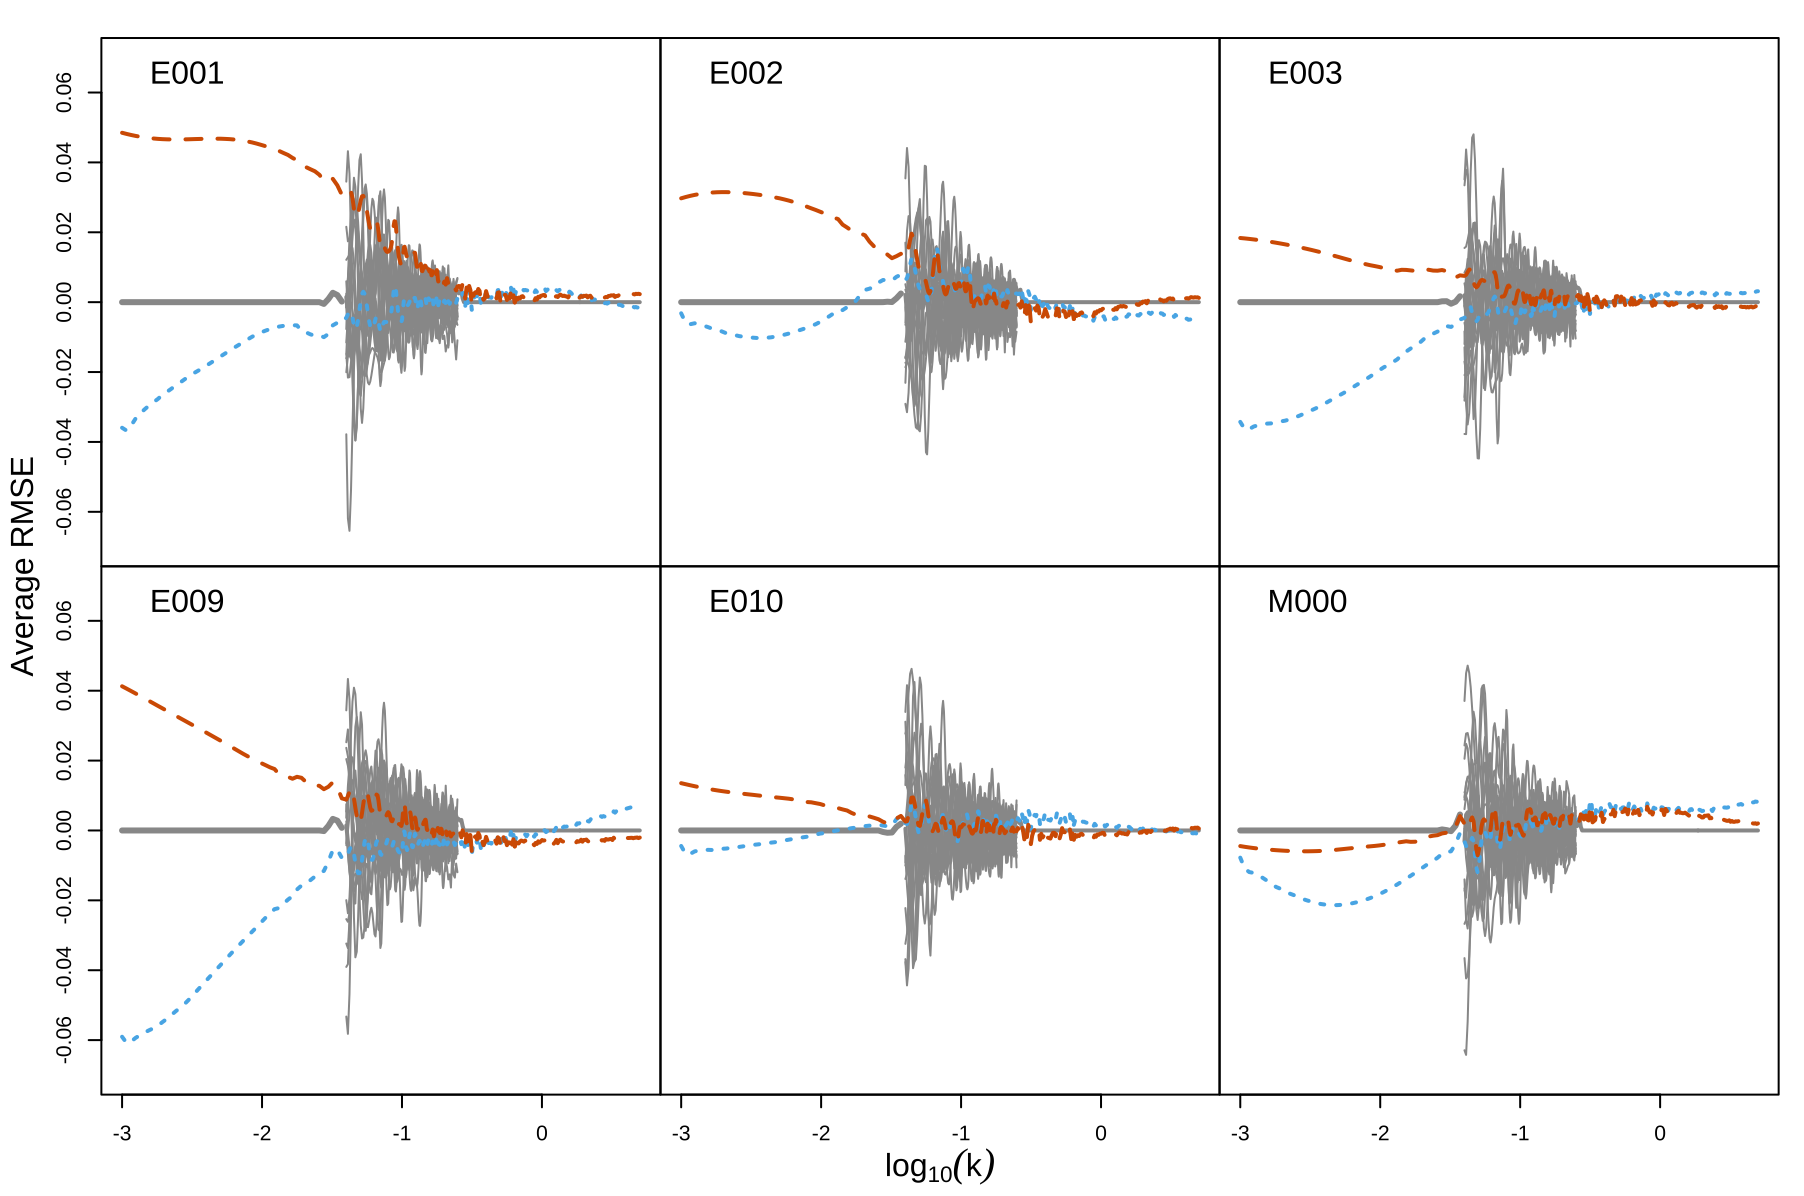
\includegraphics[width=6in]{pred_1to6.png}
    \caption{Results of all six predictions for both methods on the held-out 
    cosmologies (weighted average subtracted). CosmicEMU is dashed, DGP.HM is dotted, 
    and solid gray lines show results of held-out computer model runs.}
    \label{fig:plot_pred_1to6}
\end{figure}

\bibliographystyle{jasa}
\bibliography{references}

\end{document}
